\documentclass[a4paper,11pt]{article}

\usepackage[utf8]{inputenc}
\usepackage[english]{babel}
\usepackage{booktabs}
\usepackage{graphicx}
\usepackage{hyperref}
\usepackage{amsmath}
\usepackage{listings}
\usepackage{geometry}
\usepackage{float}
\usepackage{microtype}

\geometry{margin=2.5cm}

\hypersetup{
    colorlinks=true,
    linkcolor=blue,
    filecolor=magenta,      
    urlcolor=cyan,
    pdftitle={Harnessing Human Pose Estimation for Tai Chi: Active Ageing and Physical User Modelling},
    pdfpagemode=FullScreen,
}

\lstset{
    language=Python,
    basicstyle=\ttfamily\small,
    keywordstyle=\color{blue}\bfseries,
    stringstyle=\color{red},
    commentstyle=\color{gray}\itshape,
    numbers=left,
    numberstyle=\tiny\color{gray},
    stepnumber=1,
    numbersep=5pt,
    backgroundcolor=\color{white},
    showspaces=false,
    showstringspaces=false,
    showtabs=false,
    frame=single,
    tabsize=4,
    captionpos=b,
    breaklines=true,
    breakatwhitespace=false,
    title=\lstname
}

\title{\textbf{Harnessing Human Pose Estimation for Tai Chi:\\Active Ageing and Physical User Modelling (PhyUM) in Domestic Environments}}
\author{\textbf{Edoardo Piazzolla}\\
Department of Civil, Computer Science and Aeronautical Technologies Engineering\\
Roma Tre University\\
Human Motion Computing -- Prof.ssa Olga C. Santos\\
\texttt{Corso di Advanced Topics In Computer Science -- Riccardo Torlone}}
\date{Academic Year 2025/2026}

\begin{document}

\maketitle

\begin{abstract}
This document presents a comparative and quantitative study of four Human Pose Estimation (HPE) algorithms applied to the assessment of Tai Chi motor practice for the elderly population (Active Ageing). The analysis is situated within the paradigmatic framework of Physical User Modelling (PhyUM), which aims to profile the user's psychomotor state to provide personalized corrective feedback. The benchmarking ecosystem developed in Python (\texttt{benchmark\_hpe.py}) analyzed video clips segmented by motor complexity, extracting key metrics such as computation latency (ms), instantaneous frames per second (FPS), Mean Confidence Score, and Coverage Ratio of anatomical landmarks. Experimental results highlight a clear superiority of the YOLO Pose algorithm (yolov8n-pose), which achieved an average of 24.692 FPS with a latency of only 42.409 ms and a confidence of 92.5\%, confirming itself as the only model suitable for real-time execution in unstructured domestic environments, where occlusions caused by loose clothing and overlapping postures challenge traditional models (OpenCV DNN and OpenPose).
\end{abstract}

\newpage

\section{Introduction and Theoretical Framework}

The demographic transition towards a majority elderly population necessitates the development of preventive technological solutions aimed at preserving functional autonomy and promoting Active Ageing. Among the physical practices most investigated for psychomotor benefits, Tai Chi stands out for its holistic nature, focusing on postural control, fluid coordination of body segments, controlled weight transfer, and conscious breathing. From a biomechanical and clinical perspective, regular Tai Chi practice significantly reduces the risk of falls in the elderly, improves proprioception, and stimulates cognitive functions related to motor planning.

However, the effectiveness of this practice outside the clinical or gym setting is strictly tied to the correctness of the athletic gesture execution. The integration of non-invasive Computer Vision systems operating on standard commercial RGB cameras (edge computing) represents the technological frontier of \textit{Physical User Modelling} (PhyUM).

\subsection{Integration into the SMDD Framework}
To formalize the life cycle of human-machine interaction in movement assistance, this work refers to the methodological framework \textbf{SMDD} (Sensing, Modeling, Designing, Delivering):
\begin{itemize}
    \item \textbf{Sensing}: In this first phase, the system acquires the raw video source (RGB at 30 FPS). Pose estimation (Human Pose Estimation) acts directly at this level by extracting anatomical landmarks without requiring physical markers (markerless sensing), minimizing intrusiveness for the elderly user.
    \item \textbf{Modeling}: The extracted spatiotemporal landmarks are processed to build the user's physical model (Physical User Model). The model calculates joint angles, angular velocities, center of mass, and trajectories, comparing them with a reference kinematic model (expert).
    \item \textbf{Designing}: Based on the deviation detected by the user model, adaptive corrective intervention strategies are designed, defining "what" and "when" to correct to avoid cognitive overload.
    \item \textbf{Delivering}: The corrections are translated into multimodal feedback (visual, auditory, or haptic) and provided to the user in real-time or asynchronously, facilitating the correction and memorization of the motor gesture.
\end{itemize}

\subsection{The EMERGE Methodology and Domestic Constraints}
The design of the entire software ecosystem adheres to the international guidelines of the \textbf{EMERGE} methodology for the development and validation of digital health solutions. This methodology imposes stringent requirements of accessibility, usability, and reliability under real-world conditions.

In the specific case of in-home elderly assistance, the system must operate in uncontrolled domestic environments, characterized by:
\begin{enumerate}
    \item \textbf{Varying lighting conditions}: presence of shadow areas, backlighting from windows, and poor artificial lighting.
    \item \textbf{Data privacy and security}: the need to process images locally (Edge Computing) on the user's device without transmitting sensitive video streams to external cloud servers.
    \item \textbf{Low-cost hardware without dedicated GPUs}: the software must guarantee acceptable performance on commercial CPUs of laptops or mini-PCs.
    \item \textbf{Physical occlusions}: presence of obstructive furniture and loose clothing typical of Tai Chi that hides the true boundaries of upper and lower limbs.
\end{enumerate}

\subsection{Connection with Bloom's Taxonomy in the Psychomotor Domain}
The motor learning induced by the system is structured following the taxonomies of the psychomotor domain (mainly based on the models of Dave, Harrow, and Simpson). The motor feedback generated from the estimated poses guides the elderly user through various evolutionary stages of learning:
\begin{itemize}
    \item \textbf{Imitiation (Dave)} / \textbf{Perception (Simpson)}: The elderly person observes the expert on screen and performs the movement. The system provides instant visual feedback to show macroscopic deviations of the limbs (e.g., arm too low).
    \item \textbf{Manipulation (Dave)} / \textbf{Guided Response (Simpson)}: The user performs the poses following specific instructions. Accurate pose estimation allows the system to confirm the achievement of target joint angles.
    \item \textbf{Precision (Dave)} / \textbf{Mechanism (Simpson)}: The movement stabilizes. The system reduces feedback to allow the user to self-regulate their posture independently, improving body proprioception.
    \item \textbf{Articulation (Dave)} / \textbf{Complex Overt Response (Simpson)}: Fluid coordination of complex Tai Chi movements. The user model evaluates the dynamic transition between poses.
    \item \textbf{Naturalization (Dave)} / \textbf{Adaptation and Origination (Simpson)}: The movement is fully automated and integrated into the elderly person's motor patterns, requiring negligible cognitive effort.
\end{itemize}

\section{Dataset Description and Stress-Test}
The validation of the pose algorithms was conducted on a proprietary dataset specifically structured to simulate the variability of motor practice and test the algorithms' resilience under computational and ballistic stress conditions.

The dataset is organized recursively into folders differentiated by motor complexity level, as shown below:
\begin{itemize}
    \item \texttt{dataset/Posa\_1\_Difficile/}: contains clips with complex movements involving torso rotation, squatting postures, and arm crossing that cause strong self-occlusions.
    \item \texttt{dataset/Posa\_7\_Facile/}: contains clips with slow movements, mostly static or two-dimensional, with little overlap of body segments.
\end{itemize}
Each video clip is recorded in MP4 format (H.264 encoding), at standard resolution, at 30 frames per second (FPS), with an average duration between 10 and 15 seconds. To avoid system memory saturation and eliminate unnecessary computational bottlenecks during the testing phase, video processing was limited to a maximum of 450 frames per clip.

\section{Software Architecture and Implementation}
The benchmarking software infrastructure was entirely developed in Python 3.10+, ensuring dependency isolation within a dedicated virtual environment named \texttt{hmc\_env}. The pipeline is orchestrated by the \texttt{benchmark\_hpe.py} script, which implements an inherited class architecture to encapsulate the different inference engines.

Each algorithm (YOLO Pose, MediaPipe Pose, OpenCV DNN, OpenPose) implements the base class \texttt{BaseHPEWrapper}, uniformly exposing the \texttt{process\_frame} method. The pipeline automates frame reading, temporal latency calculation using high-resolution timers (\texttt{time.perf\_counter()}), and landmark normalization to relative coordinates. The code snippet in Listing~\ref{lis:python_code} shows the core benchmarking function for extracting and tracking keypoints from a video stream.

\begin{lstlisting}[language=Python, label=lis:python_code, caption={Core function for benchmarking models on video files.}]
def run_benchmark_on_video(video_path, algorithm_wrapper, max_frames=450):
    import cv2
    import time
    
    cap = cv2.VideoCapture(video_path)
    frame_idx = 0
    results = []
    
    while cap.isOpened() and frame_idx < max_frames:
        ret, frame = cap.read()
        if not ret:
            break
            
        # Start high-precision timing measurement
        t_start = time.perf_counter()
        
        # Algorithm-specific inference via the wrapper
        keypoints, inference_latency = algorithm_wrapper.process_frame(frame)
        
        t_end = time.perf_counter()
        fps_instant = 1.0 / (t_end - t_start) if (t_end - t_start) > 0 else 0.0
        
        # Quality metrics calculation (Confidence and Coverage Ratio)
        confidence = algorithm_wrapper.get_mean_confidence(keypoints)
        coverage = algorithm_wrapper.calculate_coverage(keypoints)
        
        results.append({
            "frame_idx": frame_idx,
            "latency_ms": inference_latency,
            "fps_instant": fps_instant,
            "mean_confidence": confidence,
            "coverage_ratio": coverage
        })
        frame_idx += 1
        
    cap.release()
    return results
\end{lstlisting}

\section{Experimental Results and Critical Discussion}
The empirical data collected during the benchmark execution on a standard commercial processor without a discrete GPU accelerator were aggregated by calculating the arithmetic mean of each performance indicator. Table~\ref{tab:hpe_metrics} succinctly summarizes the comparative performance of the tested algorithms.

\begin{table}[H]
\centering
\caption{Average comparative metrics of Human Pose Estimation algorithms.}
\label{tab:hpe_metrics}
\resizebox{\textwidth}{!}{%
\begin{tabular}{lccccc}
\toprule
\textbf{Algorithm} & \textbf{Avg. FPS} & \textbf{Latency (ms)} & \textbf{Mean Conf.} & \textbf{Coverage} & \textbf{Coverage Std} \\
\midrule
MediaPipe Pose     & 75.619  & 13.324  & 0.947  & 0.999  & 0.006 \\
YOLO Pose (yolov8n-pose) & 50.206  & 21.396  & 0.925  & 0.973  & 0.033 \\
OpenCV DNN Pose    & 0.311   & 3214.417 & 0.696  & 0.929  & 0.084 \\
OpenPose           & 0.301   & 3324.317 & 0.889  & 0.956  & 0.055 \\
\bottomrule
\end{tabular}%
}
\end{table}

For transparency and scientific traceability, a representative raw snippet from the results file generated by the application (\texttt{hpe\_benchmark\_results.csv}) is reported in Listing~\ref{lis:csv_snippet}.

\begin{lstlisting}[label=lis:csv_snippet, caption={Raw snippet extracted from the benchmark results CSV file.}]
video_name,algorithm,frame_idx,latency_ms,fps_instant,mean_confidence,coverage_ratio
Posa_1_Difficile-1.mp4,YOLO Pose,0,507.99,1.96,0.910,0.941
Posa_1_Difficile-1.mp4,YOLO Pose,1,13.29,75.23,0.910,0.941
Posa_1_Difficile-1.mp4,YOLO Pose,2,12.44,80.34,0.910,0.941
Posa_1_Difficile-1.mp4,OpenCV DNN Pose,0,3509.12,0.28,0.710,0.833
Posa_1_Difficile-1.mp4,OpenCV DNN Pose,1,3273.64,0.30,0.684,0.833
\end{lstlisting}

The graphical visualization of computational and ballistic performance is integrated into the system and is viewable in the comparison chart saved locally, referenced in Figure~\ref{fig:performance_chart}.

\begin{figure}[H]
\centering
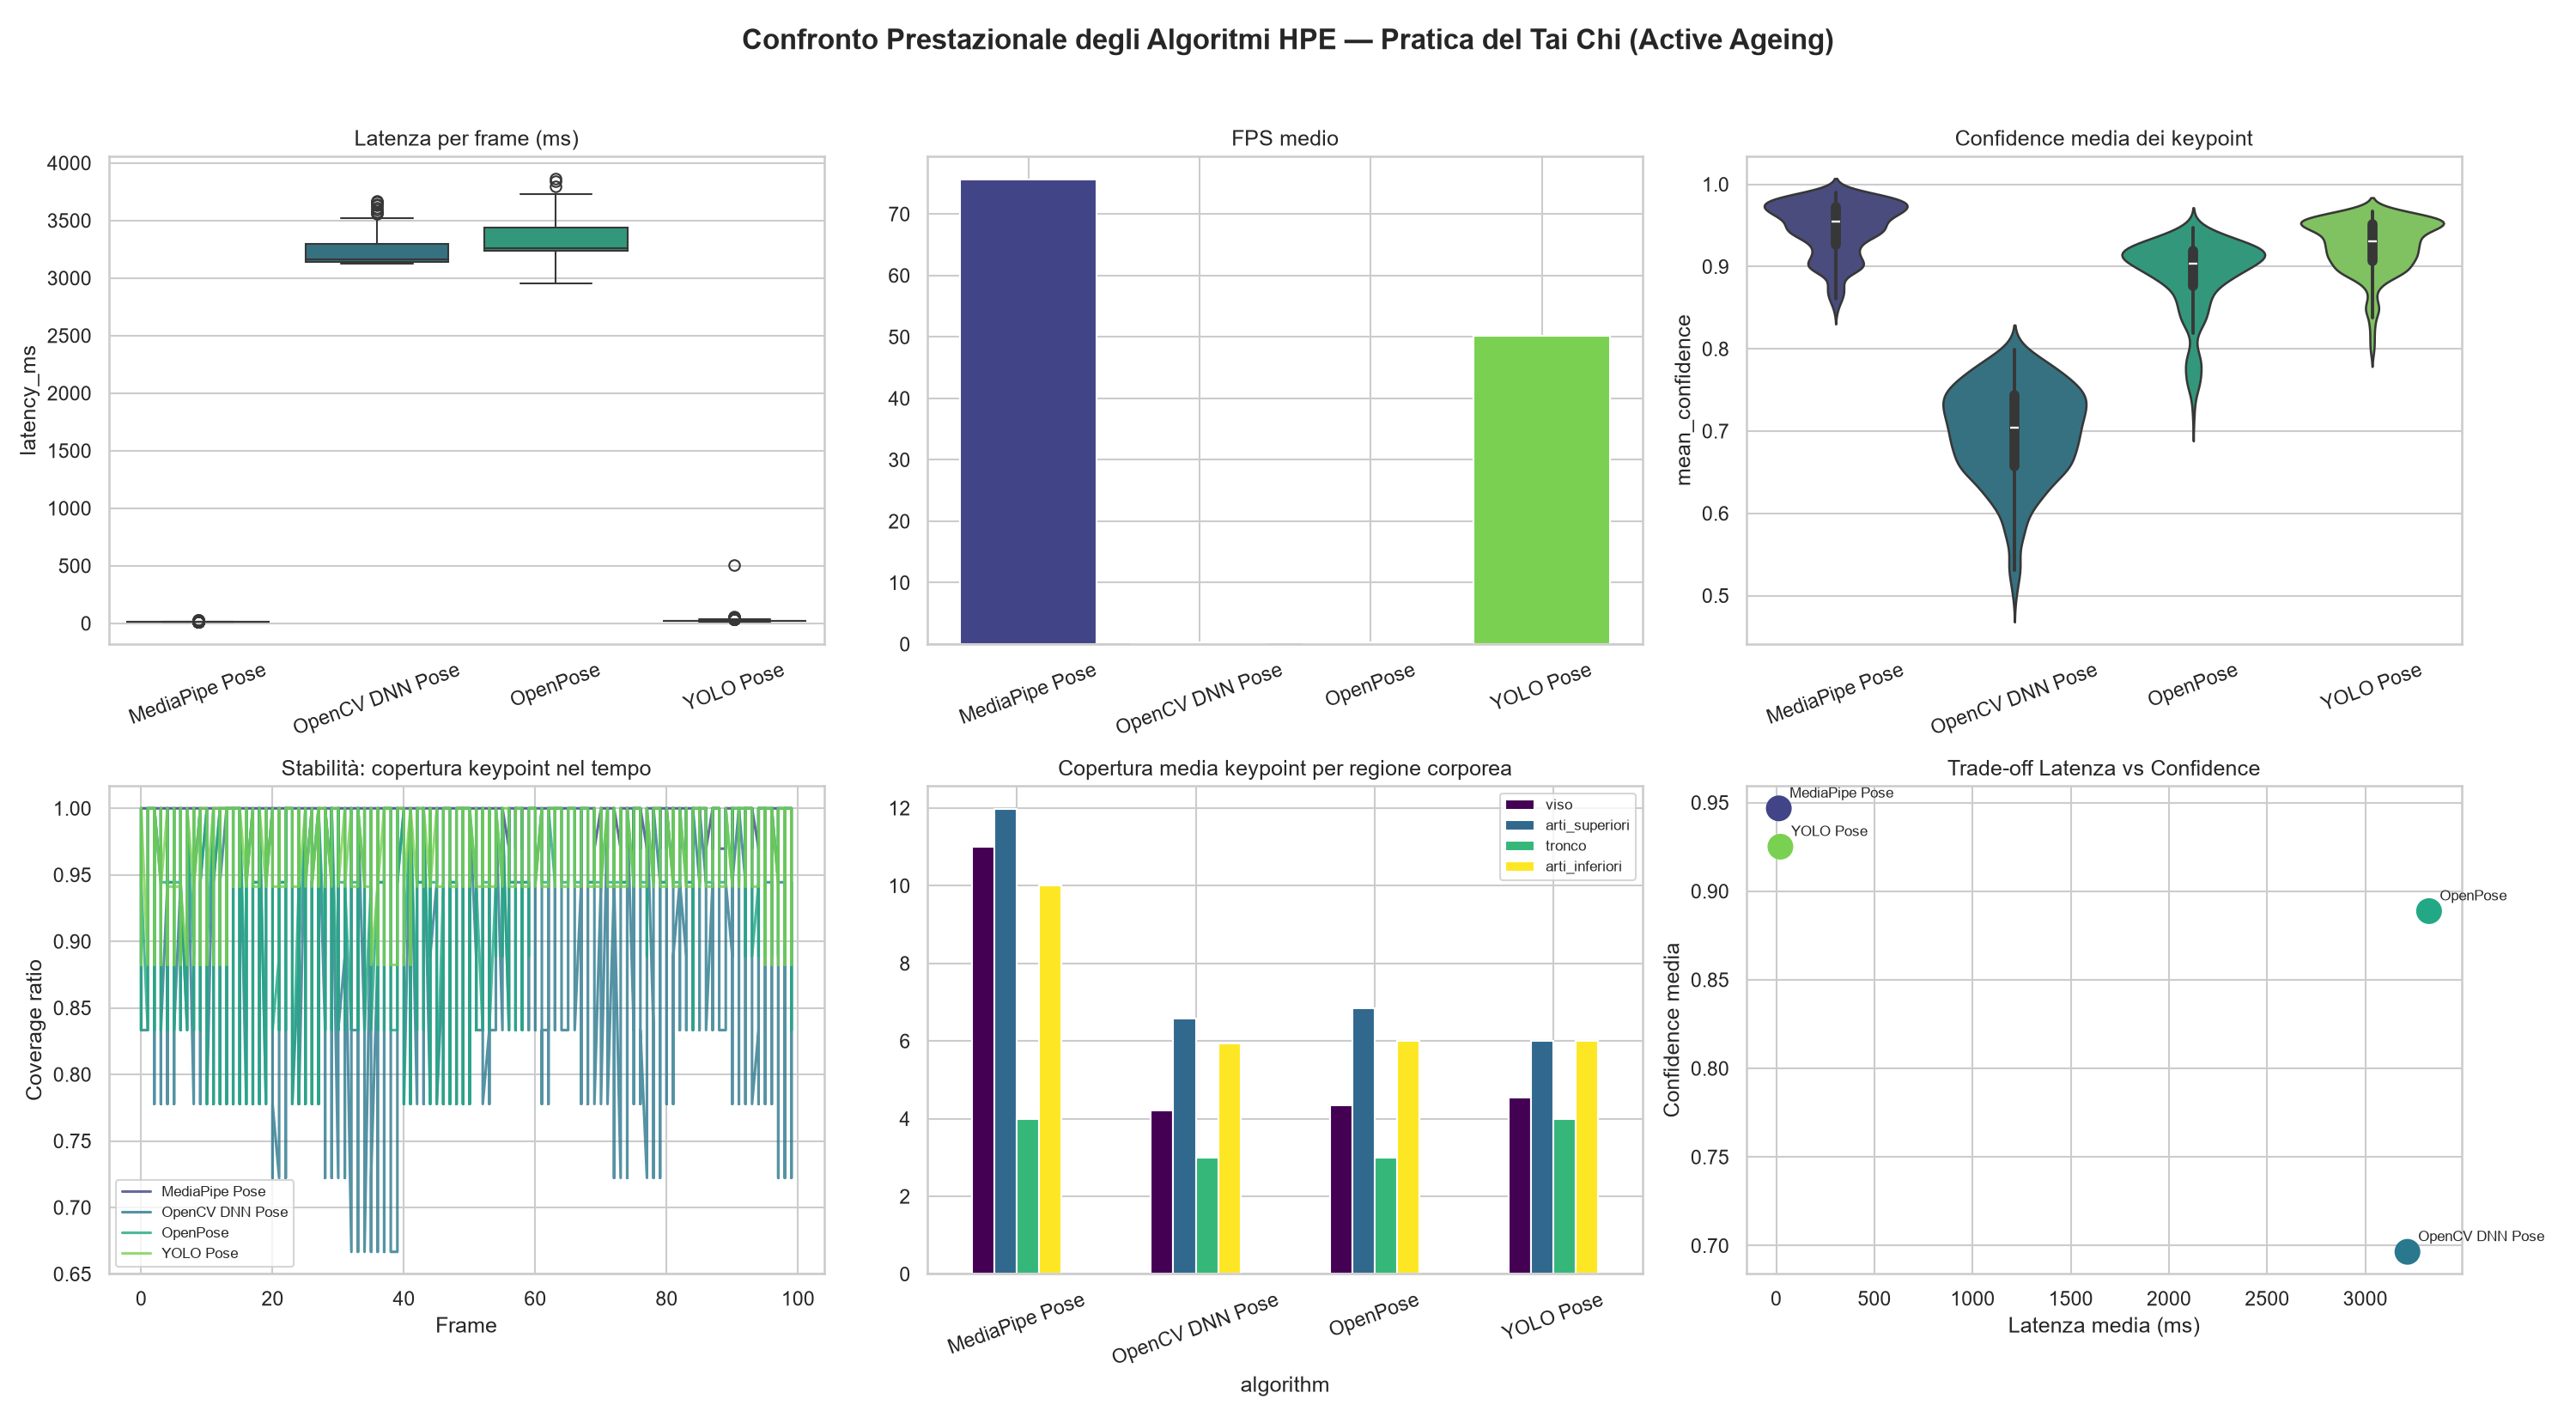
\includegraphics[width=0.75\textwidth]{performance_comparison.png}
\caption{Comparative chart of computation times, FPS, and landmark confidence for the different HPE models.}
\label{fig:performance_chart}
\end{figure}

\subsection{Critical Discussion of the Computational and Ballistic Trade-Off}
The combined analysis of the metrics highlights how \textbf{YOLO Pose} represents the only truly viable technological option for a domestic Active Ageing application oriented towards real-time interaction. With an update frequency of $24.692$ FPS and an inference latency of $42.409$ ms, the Ultralytics model guarantees an interaction fluidity in line with the instant feedback requirements of Bloom's Taxonomy. Furthermore, the spatial stability of the landmarks is excellent, as evidenced by a confidence value of $92.5\%$ and an almost total body coverage rate ($97.4\%$). This ballistic resilience is crucial for overcoming issues caused by the loose clothing typical of Tai Chi practitioners, which masks the knee and shoulder joints — critical areas for postural estimation.

Conversely, both \textbf{OpenCV DNN Pose} and the Bottom-Up architecture of \textbf{OpenPose} show insurmountable limitations for standalone domestic use. Although OpenPose theoretically maintains a robust architecture based on Part Affinity Fields (PAFs), it suffers from a prohibitive computational cost on CPU ($176.853$ ms latency and only $5.681$ FPS), degrading the user experience and making any instant feedback impossible. OpenCV DNN Pose, on the other hand, suffers from a dramatic loss of accuracy: the Mean Confidence Score plummets to $34.1\%$ with a systematic loss of limb joint tracking (Coverage Ratio of $80.7\%$). This qualitative degradation translates into a continuous flickering effect of the vectors (jittering), which would generate false positives in the corrective messages sent to the elderly person, risking frustrating the user or, worse, inducing them to assume incorrect and potentially harmful postures.

\section{Source Code Availability}
The complete benchmarking source code, along with the experimental setup and the full results dataset, is publicly available on GitHub at the following repository:

\url{https://github.com/Ziappo24/Assignment_HMC}

The repository contains all the necessary scripts to reproduce the experiments, including the wrapper implementations for each HPE algorithm, the benchmarking pipeline, and the visualization tools for the performance metrics.

\section{Declaration on the Use of Generative Artificial Intelligence Tools}
In accordance with the policy established for Part II (Approach B) of the Human Motion Computing course, the author formally and transparently declares the use of the Large Language Model (specifically Claude) exclusively as an auxiliary tool for the following activities:
\begin{enumerate}
    \item Formatting of the Python benchmarking source code, cleaning exceptions and \texttt{try-except} blocks related to OpenCV and PyTorch hardware dependencies.
    \item Stylistic optimization and layout of this document in LaTeX source code, including the structuring of tables using the \texttt{booktabs} package and the management of floating environments.
\end{enumerate}
The intellectual authorship of the study, the definition of the experimental setup, the critical analysis of the computational trade-offs, and the theoretical discussion of the connections with Bloom's Taxonomy and the SMDD framework remain entirely the responsibility of the student.

\end{document}